\documentclass[twoside]{book}

% Packages required by doxygen
\usepackage{fixltx2e}
\usepackage{calc}
\usepackage{doxygen}
\usepackage[export]{adjustbox} % also loads graphicx
\usepackage{graphicx}
\usepackage[utf8]{inputenc}
\usepackage{makeidx}
\usepackage{multicol}
\usepackage{multirow}
\PassOptionsToPackage{warn}{textcomp}
\usepackage{textcomp}
\usepackage[nointegrals]{wasysym}
\usepackage[table]{xcolor}

% Font selection
\usepackage[T1]{fontenc}
\usepackage[scaled=.90]{helvet}
\usepackage{courier}
\usepackage{amssymb}
\usepackage{sectsty}
\renewcommand{\familydefault}{\sfdefault}
\allsectionsfont{%
  \fontseries{bc}\selectfont%
  \color{darkgray}%
}
\renewcommand{\DoxyLabelFont}{%
  \fontseries{bc}\selectfont%
  \color{darkgray}%
}
\newcommand{\+}{\discretionary{\mbox{\scriptsize$\hookleftarrow$}}{}{}}

% Page & text layout
\usepackage{geometry}
\geometry{%
  a4paper,%
  top=2.5cm,%
  bottom=2.5cm,%
  left=2.5cm,%
  right=2.5cm%
}
\tolerance=750
\hfuzz=15pt
\hbadness=750
\setlength{\emergencystretch}{15pt}
\setlength{\parindent}{0cm}
\setlength{\parskip}{3ex plus 2ex minus 2ex}
\makeatletter
\renewcommand{\paragraph}{%
  \@startsection{paragraph}{4}{0ex}{-1.0ex}{1.0ex}{%
    \normalfont\normalsize\bfseries\SS@parafont%
  }%
}
\renewcommand{\subparagraph}{%
  \@startsection{subparagraph}{5}{0ex}{-1.0ex}{1.0ex}{%
    \normalfont\normalsize\bfseries\SS@subparafont%
  }%
}
\makeatother

% Headers & footers
\usepackage{fancyhdr}
\pagestyle{fancyplain}
\fancyhead[LE]{\fancyplain{}{\bfseries\thepage}}
\fancyhead[CE]{\fancyplain{}{}}
\fancyhead[RE]{\fancyplain{}{\bfseries\leftmark}}
\fancyhead[LO]{\fancyplain{}{\bfseries\rightmark}}
\fancyhead[CO]{\fancyplain{}{}}
\fancyhead[RO]{\fancyplain{}{\bfseries\thepage}}
\fancyfoot[LE]{\fancyplain{}{}}
\fancyfoot[CE]{\fancyplain{}{}}
\fancyfoot[RE]{\fancyplain{}{\bfseries\scriptsize Generated by Doxygen }}
\fancyfoot[LO]{\fancyplain{}{\bfseries\scriptsize Generated by Doxygen }}
\fancyfoot[CO]{\fancyplain{}{}}
\fancyfoot[RO]{\fancyplain{}{}}
\renewcommand{\footrulewidth}{0.4pt}
\renewcommand{\chaptermark}[1]{%
  \markboth{#1}{}%
}
\renewcommand{\sectionmark}[1]{%
  \markright{\thesection\ #1}%
}

% Indices & bibliography
\usepackage{natbib}
\usepackage[titles]{tocloft}
\setcounter{tocdepth}{3}
\setcounter{secnumdepth}{5}
\makeindex

% Hyperlinks (required, but should be loaded last)
\usepackage{ifpdf}
\ifpdf
  \usepackage[pdftex,pagebackref=true]{hyperref}
\else
  \usepackage[ps2pdf,pagebackref=true]{hyperref}
\fi
\hypersetup{%
  colorlinks=true,%
  linkcolor=blue,%
  citecolor=blue,%
  unicode%
}

% Custom commands
\newcommand{\clearemptydoublepage}{%
  \newpage{\pagestyle{empty}\cleardoublepage}%
}

\usepackage{caption}
\captionsetup{labelsep=space,justification=centering,font={bf},singlelinecheck=off,skip=4pt,position=top}

%===== C O N T E N T S =====

\begin{document}

% Titlepage & ToC
\hypersetup{pageanchor=false,
             bookmarksnumbered=true,
             pdfencoding=unicode
            }
\pagenumbering{roman}
\begin{titlepage}
\vspace*{7cm}
\begin{center}%
{\Large Tubes O\+OP }\\
\vspace*{1cm}
{\large Generated by Doxygen 1.8.11}\\
\end{center}
\end{titlepage}
\clearemptydoublepage
\tableofcontents
\clearemptydoublepage
\pagenumbering{arabic}
\hypersetup{pageanchor=true}

%--- Begin generated contents ---
\chapter{Hierarchical Index}
\section{Class Hierarchy}
This inheritance list is sorted roughly, but not completely, alphabetically\+:\begin{DoxyCompactList}
\item \contentsline{section}{board}{\pageref{classboard}}{}
\item \contentsline{section}{list}{\pageref{classlist}}{}
\item \contentsline{section}{makhluk}{\pageref{classmakhluk}}{}
\begin{DoxyCompactList}
\item \contentsline{section}{herbivora}{\pageref{classherbivora}}{}
\begin{DoxyCompactList}
\item \contentsline{section}{zebra}{\pageref{classzebra}}{}
\end{DoxyCompactList}
\item \contentsline{section}{karnivora}{\pageref{classkarnivora}}{}
\begin{DoxyCompactList}
\item \contentsline{section}{singa}{\pageref{classsinga}}{}
\end{DoxyCompactList}
\end{DoxyCompactList}
\item \contentsline{section}{list\+:\+:node}{\pageref{structlist_1_1node}}{}
\item \contentsline{section}{Point}{\pageref{class_point}}{}
\item thread\begin{DoxyCompactList}
\item \contentsline{section}{guarded\+\_\+thread}{\pageref{structguarded__thread}}{}
\end{DoxyCompactList}
\end{DoxyCompactList}

\chapter{Class Index}
\section{Class List}
Here are the classes, structs, unions and interfaces with brief descriptions\+:\begin{DoxyCompactList}
\item\contentsline{section}{\hyperlink{classboard}{board} }{\pageref{classboard}}{}
\item\contentsline{section}{\hyperlink{structguarded__thread}{guarded\+\_\+thread} }{\pageref{structguarded__thread}}{}
\item\contentsline{section}{\hyperlink{classherbivora}{herbivora} }{\pageref{classherbivora}}{}
\item\contentsline{section}{\hyperlink{classkarnivora}{karnivora} }{\pageref{classkarnivora}}{}
\item\contentsline{section}{\hyperlink{classlist}{list} }{\pageref{classlist}}{}
\item\contentsline{section}{\hyperlink{classmakhluk}{makhluk} \\*Abstract Class -\/ tidak bisa dibuat objeknya }{\pageref{classmakhluk}}{}
\item\contentsline{section}{\hyperlink{structlist_1_1node}{list\+::node} \\*Struktur sebuah node list }{\pageref{structlist_1_1node}}{}
\item\contentsline{section}{\hyperlink{class_point}{Point} }{\pageref{class_point}}{}
\item\contentsline{section}{\hyperlink{classsinga}{singa} }{\pageref{classsinga}}{}
\item\contentsline{section}{\hyperlink{classzebra}{zebra} }{\pageref{classzebra}}{}
\end{DoxyCompactList}

\chapter{Class Documentation}
\hypertarget{classboard}{}\section{board Class Reference}
\label{classboard}\index{board@{board}}
\subsection*{Public Member Functions}
\begin{DoxyCompactItemize}
\item 
void {\bfseries printboard} ()\hypertarget{classboard_a6e982dd9f066e8bdd47e62dcb2b58d4d}{}\label{classboard_a6e982dd9f066e8bdd47e62dcb2b58d4d}

\item 
void {\bfseries tambah} (\hyperlink{classmakhluk}{makhluk} \&)\hypertarget{classboard_ae032573539a2aaecc8416ebde30d4ccd}{}\label{classboard_ae032573539a2aaecc8416ebde30d4ccd}

\item 
void {\bfseries move} (\hyperlink{classmakhluk}{makhluk} \&)\hypertarget{classboard_abc546e7b17944d8135f101776cb12be8}{}\label{classboard_abc546e7b17944d8135f101776cb12be8}

\item 
void {\bfseries hapus} (\hyperlink{classmakhluk}{makhluk} \&)\hypertarget{classboard_a1b16f7efa467fd465477181d8daf12bd}{}\label{classboard_a1b16f7efa467fd465477181d8daf12bd}

\item 
void {\bfseries tofile} ()\hypertarget{classboard_a541f795cb1106060602b381723c3bd7b}{}\label{classboard_a541f795cb1106060602b381723c3bd7b}

\end{DoxyCompactItemize}
\subsection*{Protected Attributes}
\begin{DoxyCompactItemize}
\item 
const int {\bfseries sizex} = 30\hypertarget{classboard_a3da53c304c897ae66fa021d153c6e175}{}\label{classboard_a3da53c304c897ae66fa021d153c6e175}

\item 
const int {\bfseries sizey} = 30\hypertarget{classboard_a2489f58a0ee5032a5ba2895cd3852a47}{}\label{classboard_a2489f58a0ee5032a5ba2895cd3852a47}

\item 
char {\bfseries isi} \mbox{[}30\mbox{]}\mbox{[}30\mbox{]}\hypertarget{classboard_af9c1f553b476ba832d7aafc33cc4cbfc}{}\label{classboard_af9c1f553b476ba832d7aafc33cc4cbfc}

\end{DoxyCompactItemize}


The documentation for this class was generated from the following files\+:\begin{DoxyCompactItemize}
\item 
board.\+h\item 
board.\+cpp\end{DoxyCompactItemize}

\hypertarget{structguarded__thread}{}\section{guarded\+\_\+thread Struct Reference}
\label{structguarded__thread}\index{guarded\+\_\+thread@{guarded\+\_\+thread}}
Inheritance diagram for guarded\+\_\+thread\+:\begin{figure}[H]
\begin{center}
\leavevmode
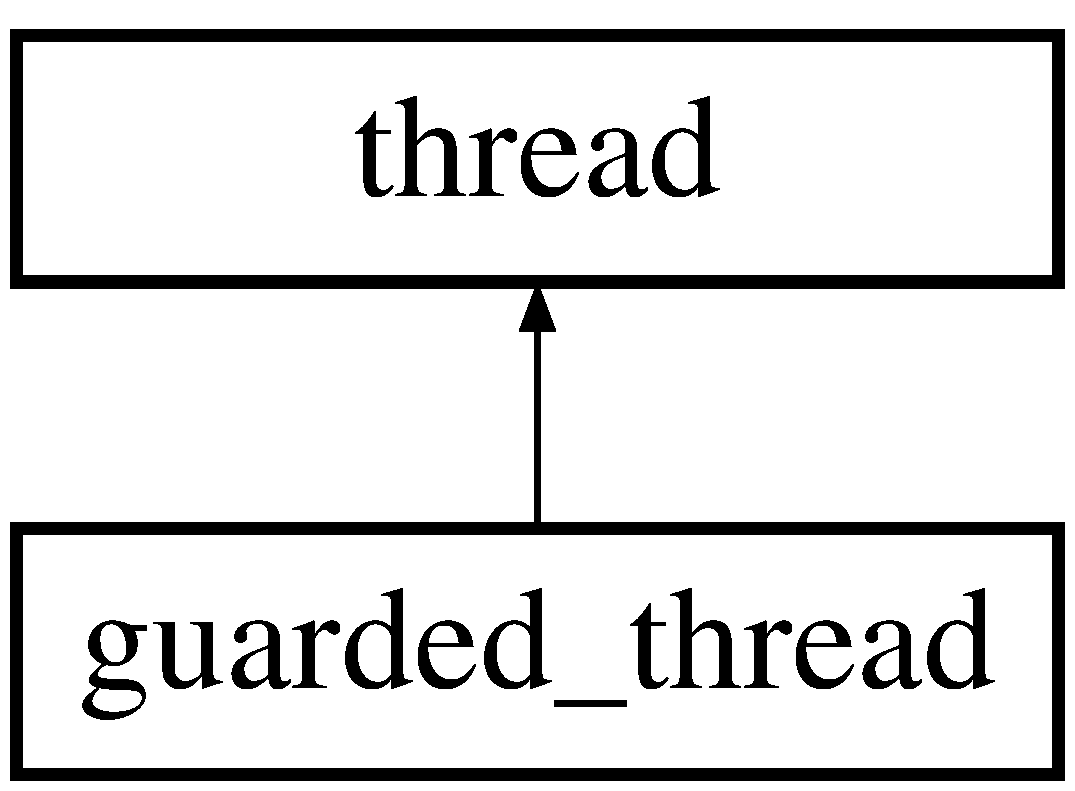
\includegraphics[height=2.000000cm]{structguarded__thread}
\end{center}
\end{figure}


The documentation for this struct was generated from the following file\+:\begin{DoxyCompactItemize}
\item 
guarded\+\_\+thread.\+h\end{DoxyCompactItemize}

\hypertarget{classherbivora}{}\section{herbivora Class Reference}
\label{classherbivora}\index{herbivora@{herbivora}}
Inheritance diagram for herbivora\+:\begin{figure}[H]
\begin{center}
\leavevmode
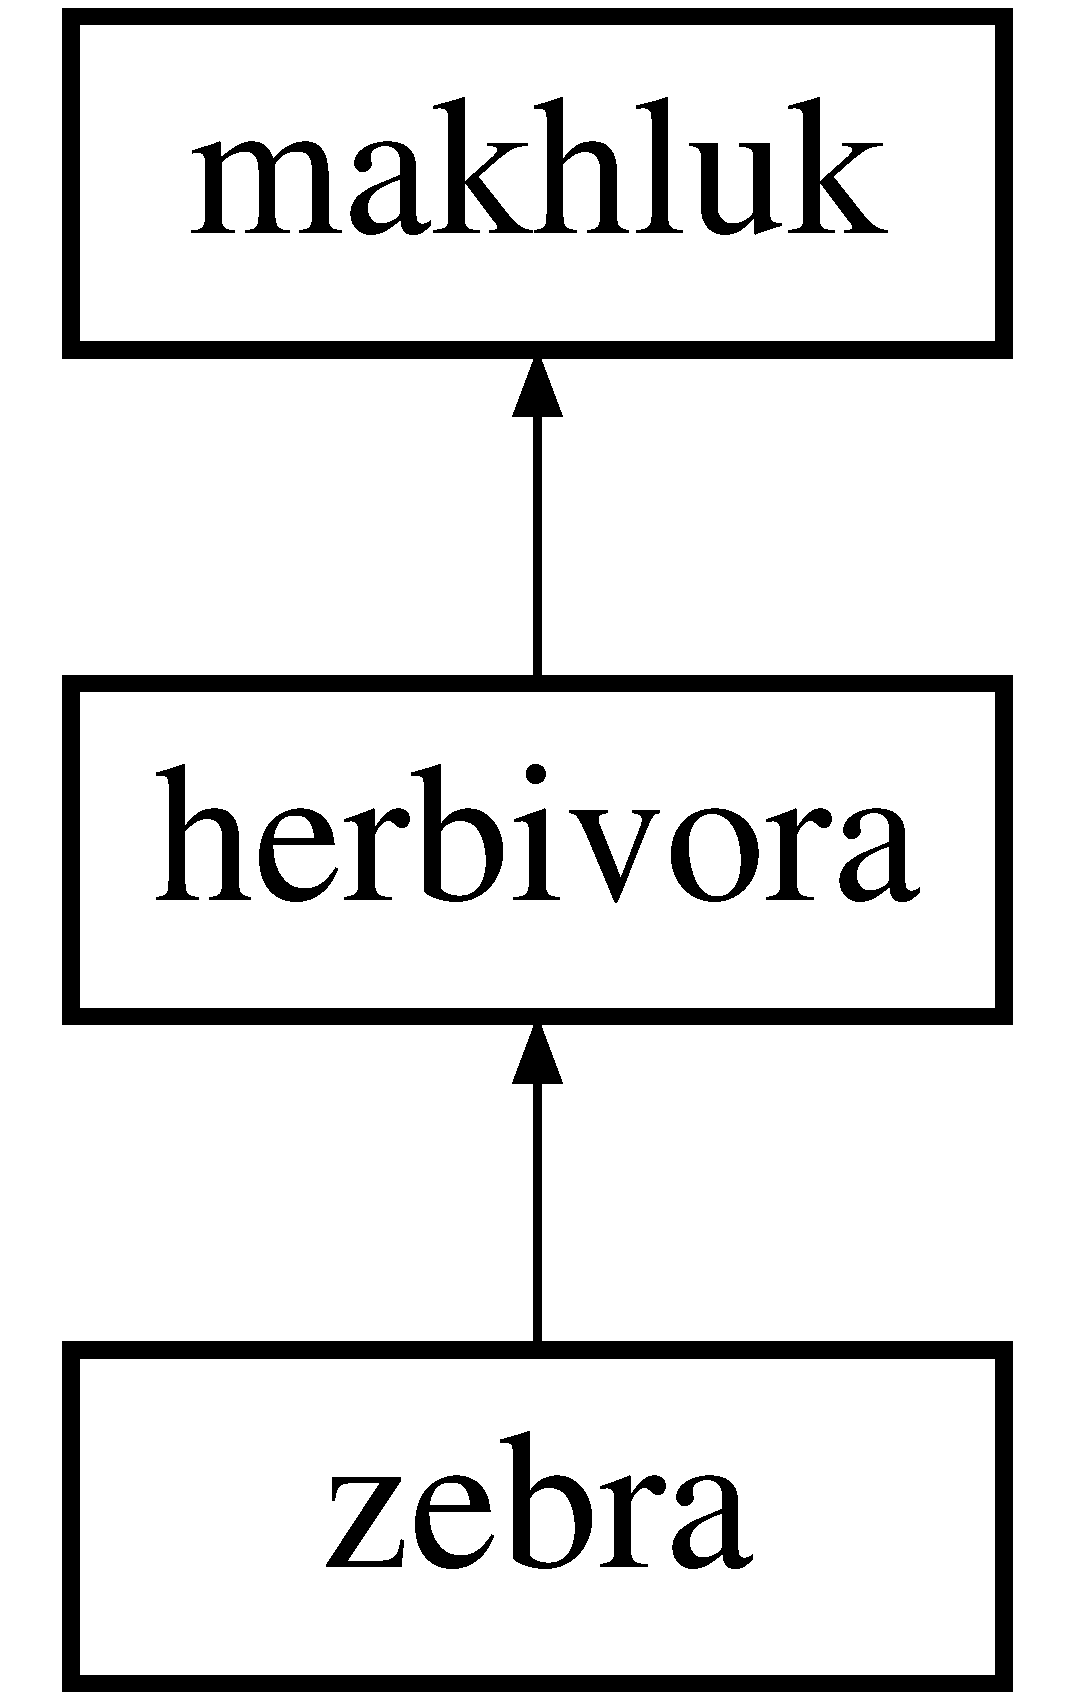
\includegraphics[height=3.000000cm]{classherbivora}
\end{center}
\end{figure}
\subsection*{Public Member Functions}
\begin{DoxyCompactItemize}
\item 
virtual void \hyperlink{classherbivora_ad4ee54fdd628e1863f8bc11289afa5fc}{makan} ()=0\hypertarget{classherbivora_ad4ee54fdd628e1863f8bc11289afa5fc}{}\label{classherbivora_ad4ee54fdd628e1863f8bc11289afa5fc}

\begin{DoxyCompactList}\small\item\em memakan objek lain -\/ kelas turunannya harus mengimplementasikan ini \end{DoxyCompactList}\item 
virtual void {\bfseries sembunyi} ()\hypertarget{classherbivora_ab2f643594070089bf9b0fdd556e4d1c4}{}\label{classherbivora_ab2f643594070089bf9b0fdd556e4d1c4}

\item 
virtual void \hyperlink{classherbivora_af95061149dcaa995cf00471181f5b9cb}{bergerak} ()\hypertarget{classherbivora_af95061149dcaa995cf00471181f5b9cb}{}\label{classherbivora_af95061149dcaa995cf00471181f5b9cb}

\begin{DoxyCompactList}\small\item\em objek turunan makhluk berpindah ke koordinat lain \end{DoxyCompactList}\item 
virtual int \hyperlink{classherbivora_a2d486857a57ee4b56f907c9a0b528a28}{getlapar} ()\hypertarget{classherbivora_a2d486857a57ee4b56f907c9a0b528a28}{}\label{classherbivora_a2d486857a57ee4b56f907c9a0b528a28}

\begin{DoxyCompactList}\small\item\em mendapatkan level kelaparan sebuah objek turunan makhluk \end{DoxyCompactList}\end{DoxyCompactItemize}
\subsection*{Protected Attributes}
\begin{DoxyCompactItemize}
\item 
int {\bfseries mlapar}\hypertarget{classherbivora_aaec5704f5e23be6e458aabf3029b11e3}{}\label{classherbivora_aaec5704f5e23be6e458aabf3029b11e3}

\end{DoxyCompactItemize}


The documentation for this class was generated from the following files\+:\begin{DoxyCompactItemize}
\item 
herbivora.\+h\item 
herbivora.\+cpp\end{DoxyCompactItemize}

\hypertarget{classkarnivora}{}\section{karnivora Class Reference}
\label{classkarnivora}\index{karnivora@{karnivora}}
Inheritance diagram for karnivora\+:\begin{figure}[H]
\begin{center}
\leavevmode
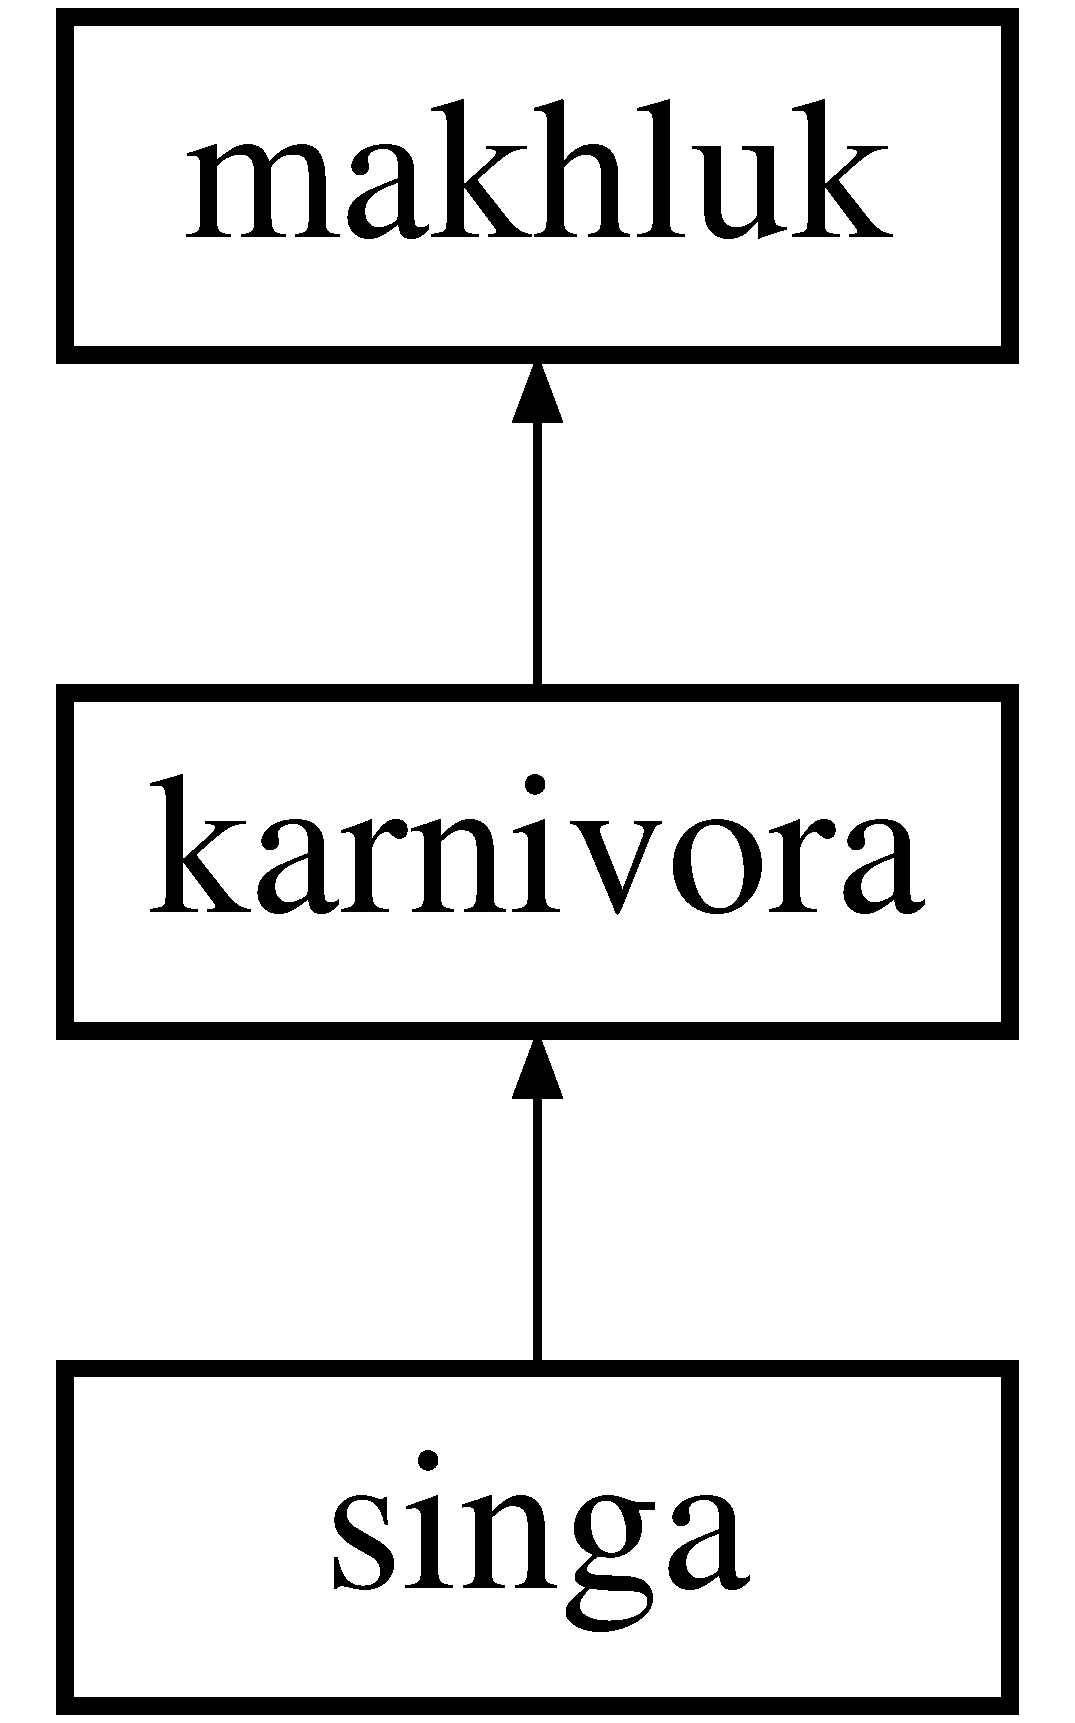
\includegraphics[height=3.000000cm]{classkarnivora}
\end{center}
\end{figure}
\subsection*{Public Member Functions}
\begin{DoxyCompactItemize}
\item 
virtual void \hyperlink{classkarnivora_a80ebba77a163a8412be6f05ac0000a6b}{makan} ()=0\hypertarget{classkarnivora_a80ebba77a163a8412be6f05ac0000a6b}{}\label{classkarnivora_a80ebba77a163a8412be6f05ac0000a6b}

\begin{DoxyCompactList}\small\item\em memakan objek lain -\/ kelas turunannya harus mengimplementasikan ini \end{DoxyCompactList}\item 
void {\bfseries lihat} ()\hypertarget{classkarnivora_a14a6b8728c4c8e0310cf4ccbff9b5d63}{}\label{classkarnivora_a14a6b8728c4c8e0310cf4ccbff9b5d63}

\item 
void \hyperlink{classkarnivora_a9ba6d3ddb24b0266aa40d8a2555cd11c}{bergerak} ()\hypertarget{classkarnivora_a9ba6d3ddb24b0266aa40d8a2555cd11c}{}\label{classkarnivora_a9ba6d3ddb24b0266aa40d8a2555cd11c}

\begin{DoxyCompactList}\small\item\em objek turunan makhluk berpindah ke koordinat lain \end{DoxyCompactList}\item 
int \hyperlink{classkarnivora_a33ff754594ab65d83eaf6dd7bb30d8a5}{getlapar} ()\hypertarget{classkarnivora_a33ff754594ab65d83eaf6dd7bb30d8a5}{}\label{classkarnivora_a33ff754594ab65d83eaf6dd7bb30d8a5}

\begin{DoxyCompactList}\small\item\em mendapatkan level kelaparan sebuah objek turunan makhluk \end{DoxyCompactList}\item 
void \hyperlink{classkarnivora_aefc7c8260e5f282f63f5eff0c08e266c}{printstatmakhluk} ()\hypertarget{classkarnivora_aefc7c8260e5f282f63f5eff0c08e266c}{}\label{classkarnivora_aefc7c8260e5f282f63f5eff0c08e266c}

\begin{DoxyCompactList}\small\item\em menampilkan semua status makhluk \end{DoxyCompactList}\end{DoxyCompactItemize}
\subsection*{Protected Attributes}
\begin{DoxyCompactItemize}
\item 
int {\bfseries mlapar}\hypertarget{classkarnivora_a0b48304fede2005274cf787d765107d3}{}\label{classkarnivora_a0b48304fede2005274cf787d765107d3}

\item 
int {\bfseries jenismakanan}\hypertarget{classkarnivora_a21c9dcfc494dcd1bad9edd3facc7cecb}{}\label{classkarnivora_a21c9dcfc494dcd1bad9edd3facc7cecb}

\end{DoxyCompactItemize}


The documentation for this class was generated from the following files\+:\begin{DoxyCompactItemize}
\item 
karnivora.\+h\item 
karnivora.\+cpp\end{DoxyCompactItemize}

\hypertarget{classlist}{}\section{list Class Reference}
\label{classlist}\index{list@{list}}
\subsection*{Classes}
\begin{DoxyCompactItemize}
\item 
struct \hyperlink{structlist_1_1node}{node}
\begin{DoxyCompactList}\small\item\em struktur sebuah node list \end{DoxyCompactList}\end{DoxyCompactItemize}
\subsection*{Public Member Functions}
\begin{DoxyCompactItemize}
\item 
\hyperlink{classlist_a223ecca7c96ef287c1e647493a32fbf6}{list} ()
\begin{DoxyCompactList}\small\item\em constructor \end{DoxyCompactList}\item 
\hyperlink{classlist_a72eaabb03a048506432f8d167db12524}{$\sim$list} ()\hypertarget{classlist_a72eaabb03a048506432f8d167db12524}{}\label{classlist_a72eaabb03a048506432f8d167db12524}

\begin{DoxyCompactList}\small\item\em destructor \end{DoxyCompactList}\item 
int {\bfseries is\+Empty} ()\hypertarget{classlist_a890b680743d30859bf0b5dbbdc3d8544}{}\label{classlist_a890b680743d30859bf0b5dbbdc3d8544}

\item 
int {\bfseries is\+One\+Elmt} ()\hypertarget{classlist_a4c10a6850cbbffa7c652868e973e0625}{}\label{classlist_a4c10a6850cbbffa7c652868e973e0625}

\item 
struct \hyperlink{structlist_1_1node}{list\+::node} $\ast$ {\bfseries search\+Makhluk} (struct \hyperlink{structlist_1_1node}{list\+::node} $\ast$, string)\hypertarget{classlist_ab629e99e39c4430c65806a3ec1dc6bb6}{}\label{classlist_ab629e99e39c4430c65806a3ec1dc6bb6}

\item 
void {\bfseries add\+Node} (string s, int i)\hypertarget{classlist_ad933a0b859de2f967649c2be0214b3fc}{}\label{classlist_ad933a0b859de2f967649c2be0214b3fc}

\item 
void {\bfseries delete\+Node} (struct \hyperlink{structlist_1_1node}{list\+::node} $\ast$)\hypertarget{classlist_ac1993ef62ac339a9d7e60baaf96b5062}{}\label{classlist_ac1993ef62ac339a9d7e60baaf96b5062}

\item 
void {\bfseries print\+List} (struct \hyperlink{structlist_1_1node}{list\+::node} $\ast$)\hypertarget{classlist_aa4cd401b862217d241c396311fc9a45e}{}\label{classlist_aa4cd401b862217d241c396311fc9a45e}

\end{DoxyCompactItemize}
\subsection*{Public Attributes}
\begin{DoxyCompactItemize}
\item 
struct \hyperlink{structlist_1_1node}{list\+::node} $\ast$ {\bfseries head}\hypertarget{classlist_a4f239eff5de08cc69b80e112ebf5da68}{}\label{classlist_a4f239eff5de08cc69b80e112ebf5da68}

\item 
struct \hyperlink{structlist_1_1node}{list\+::node} $\ast$ {\bfseries tail}\hypertarget{classlist_ab8bbd944fee9f635d3f8a7387a23efaf}{}\label{classlist_ab8bbd944fee9f635d3f8a7387a23efaf}

\end{DoxyCompactItemize}


\subsection{Constructor \& Destructor Documentation}
\index{list@{list}!list@{list}}
\index{list@{list}!list@{list}}
\subsubsection[{\texorpdfstring{list()}{list()}}]{\setlength{\rightskip}{0pt plus 5cm}list\+::list (
\begin{DoxyParamCaption}
{}
\end{DoxyParamCaption}
)}\hypertarget{classlist_a223ecca7c96ef287c1e647493a32fbf6}{}\label{classlist_a223ecca7c96ef287c1e647493a32fbf6}


constructor 

---head menunjuk address node pertama ---tail menunjuk address node terakhir 

The documentation for this class was generated from the following files\+:\begin{DoxyCompactItemize}
\item 
list.\+h\item 
list.\+cpp\end{DoxyCompactItemize}

\hypertarget{classmakhluk}{}\section{makhluk Class Reference}
\label{classmakhluk}\index{makhluk@{makhluk}}


Abstract Class -\/ tidak bisa dibuat objeknya.  




{\ttfamily \#include $<$makhluk.\+h$>$}

Inheritance diagram for makhluk\+:\begin{figure}[H]
\begin{center}
\leavevmode
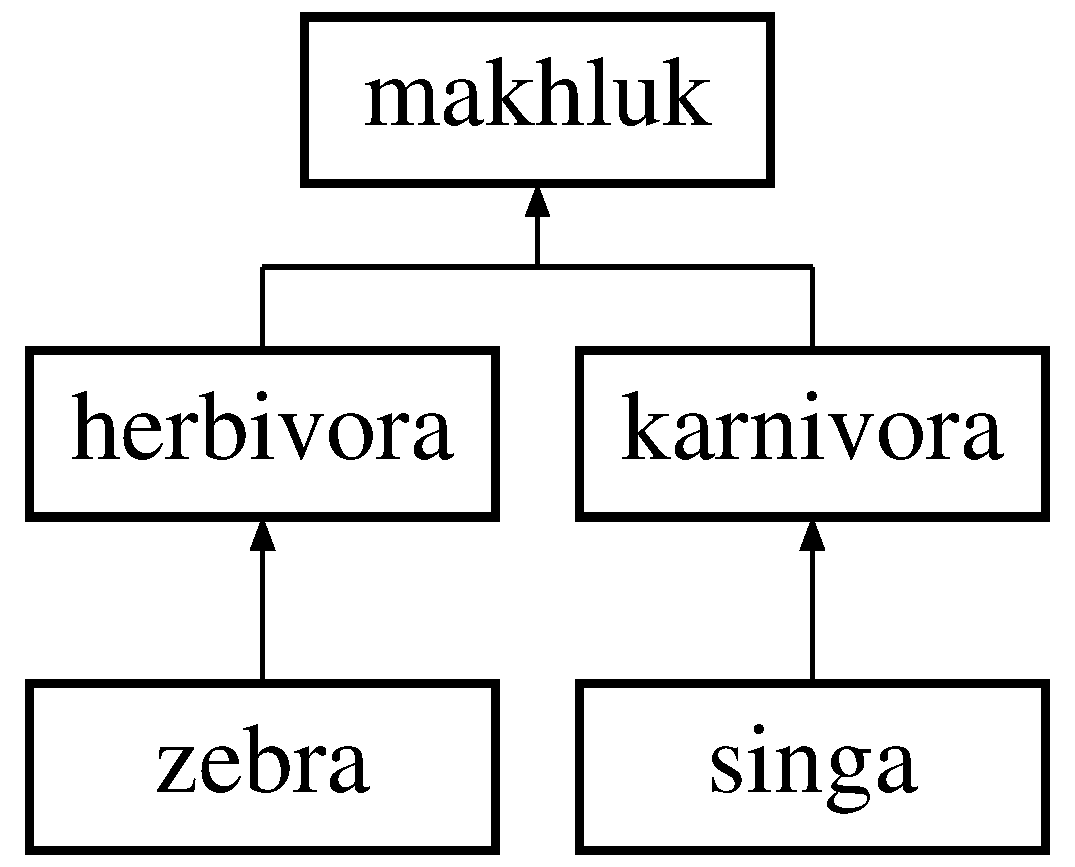
\includegraphics[height=3.000000cm]{classmakhluk}
\end{center}
\end{figure}
\subsection*{Public Member Functions}
\begin{DoxyCompactItemize}
\item 
\hyperlink{classmakhluk_adbc575116661f7837693c1038aa16c40}{makhluk} ()\hypertarget{classmakhluk_adbc575116661f7837693c1038aa16c40}{}\label{classmakhluk_adbc575116661f7837693c1038aa16c40}

\begin{DoxyCompactList}\small\item\em konstruktor \end{DoxyCompactList}\item 
virtual \hyperlink{classmakhluk_a29be824daa6c805d6259a2db6870b943}{$\sim$makhluk} ()\hypertarget{classmakhluk_a29be824daa6c805d6259a2db6870b943}{}\label{classmakhluk_a29be824daa6c805d6259a2db6870b943}

\begin{DoxyCompactList}\small\item\em destruktor \end{DoxyCompactList}\item 
virtual void \hyperlink{classmakhluk_a0b4d95d9f0dc0662360064e31d3a986c}{bergerak} ()\hypertarget{classmakhluk_a0b4d95d9f0dc0662360064e31d3a986c}{}\label{classmakhluk_a0b4d95d9f0dc0662360064e31d3a986c}

\begin{DoxyCompactList}\small\item\em objek turunan makhluk berpindah ke koordinat lain \end{DoxyCompactList}\item 
virtual void \hyperlink{classmakhluk_a36493787b5e974f2f6d3da7b260ac9cf}{makan} ()=0\hypertarget{classmakhluk_a36493787b5e974f2f6d3da7b260ac9cf}{}\label{classmakhluk_a36493787b5e974f2f6d3da7b260ac9cf}

\begin{DoxyCompactList}\small\item\em memakan objek lain -\/ kelas turunannya harus mengimplementasikan ini \end{DoxyCompactList}\item 
virtual int \hyperlink{classmakhluk_a9e348a59401f5e66aae435d6b73d0481}{getlapar} ()=0\hypertarget{classmakhluk_a9e348a59401f5e66aae435d6b73d0481}{}\label{classmakhluk_a9e348a59401f5e66aae435d6b73d0481}

\begin{DoxyCompactList}\small\item\em mendapatkan level kelaparan sebuah objek turunan makhluk \end{DoxyCompactList}\item 
\hyperlink{class_point}{Point} \hyperlink{classmakhluk_a484f54517aaf27f21e6414c7f5fadd7b}{getlok} ()\hypertarget{classmakhluk_a484f54517aaf27f21e6414c7f5fadd7b}{}\label{classmakhluk_a484f54517aaf27f21e6414c7f5fadd7b}

\begin{DoxyCompactList}\small\item\em mendapatkan lokasi (x, y) sebuah objek turunan makhluk di bidang \end{DoxyCompactList}\item 
void \hyperlink{classmakhluk_a8dd010db343f225fe4dc01b36761c888}{printlok} ()\hypertarget{classmakhluk_a8dd010db343f225fe4dc01b36761c888}{}\label{classmakhluk_a8dd010db343f225fe4dc01b36761c888}

\begin{DoxyCompactList}\small\item\em menampilkan lokasi (x, y) sebuah objek turunan makhluk di bidang \end{DoxyCompactList}\item 
virtual void \hyperlink{classmakhluk_a87083e725642bb622827304d146242d2}{printstatmakhluk} ()\hypertarget{classmakhluk_a87083e725642bb622827304d146242d2}{}\label{classmakhluk_a87083e725642bb622827304d146242d2}

\begin{DoxyCompactList}\small\item\em menampilkan semua status makhluk \end{DoxyCompactList}\end{DoxyCompactItemize}
\subsection*{Protected Attributes}
\begin{DoxyCompactItemize}
\item 
int {\bfseries dt}\hypertarget{classmakhluk_a0bbc6dba97261e511bb9a407f5081f83}{}\label{classmakhluk_a0bbc6dba97261e511bb9a407f5081f83}

\item 
int \hyperlink{classmakhluk_add10f9625fcea85f3871ad2996808c0f}{umur}\hypertarget{classmakhluk_add10f9625fcea85f3871ad2996808c0f}{}\label{classmakhluk_add10f9625fcea85f3871ad2996808c0f}

\begin{DoxyCompactList}\small\item\em selang waktu gerak sebuah objek turunan makhluk \end{DoxyCompactList}\item 
int {\bfseries power}\hypertarget{classmakhluk_a43298c45f6d7353bb3f0ddd45048da1f}{}\label{classmakhluk_a43298c45f6d7353bb3f0ddd45048da1f}

\item 
int \hyperlink{classmakhluk_a6977ae3b2d7a83f823498c04326c2979}{arah}\hypertarget{classmakhluk_a6977ae3b2d7a83f823498c04326c2979}{}\label{classmakhluk_a6977ae3b2d7a83f823498c04326c2979}

\begin{DoxyCompactList}\small\item\em kekuatan sebuah objek turunan makhluk \end{DoxyCompactList}\item 
\hyperlink{class_point}{Point} \hyperlink{classmakhluk_ae52cf4323ddd35bf9c15e9598131167e}{P}\hypertarget{classmakhluk_ae52cf4323ddd35bf9c15e9598131167e}{}\label{classmakhluk_ae52cf4323ddd35bf9c15e9598131167e}

\begin{DoxyCompactList}\small\item\em arah gerak sebuah objek turunan makhluk \end{DoxyCompactList}\end{DoxyCompactItemize}


\subsection{Detailed Description}
Abstract Class -\/ tidak bisa dibuat objeknya. 

The documentation for this class was generated from the following files\+:\begin{DoxyCompactItemize}
\item 
makhluk.\+h\item 
makhluk.\+cpp\end{DoxyCompactItemize}

\hypertarget{structlist_1_1node}{}\section{list\+:\+:node Struct Reference}
\label{structlist_1_1node}\index{list\+::node@{list\+::node}}


struktur sebuah node list  




{\ttfamily \#include $<$list.\+h$>$}

\subsection*{Public Attributes}
\begin{DoxyCompactItemize}
\item 
string {\bfseries nama\+\_\+makhluk}\hypertarget{structlist_1_1node_a06f92cd10b0f1273f38dd9d69796688f}{}\label{structlist_1_1node_a06f92cd10b0f1273f38dd9d69796688f}

\item 
struct \hyperlink{structlist_1_1node}{node} $\ast$ {\bfseries next}\hypertarget{structlist_1_1node_a3fef0f498c6c1cf8e8cc9cf92edcc664}{}\label{structlist_1_1node_a3fef0f498c6c1cf8e8cc9cf92edcc664}

\end{DoxyCompactItemize}


\subsection{Detailed Description}
struktur sebuah node list 

The documentation for this struct was generated from the following file\+:\begin{DoxyCompactItemize}
\item 
list.\+h\end{DoxyCompactItemize}

\hypertarget{class_point}{}\section{Point Class Reference}
\label{class_point}\index{Point@{Point}}
\subsection*{Public Member Functions}
\begin{DoxyCompactItemize}
\item 
{\bfseries Point} (int \+\_\+X, int \+\_\+Y)\hypertarget{class_point_a581ce64df5e5e16cf9e31bdbf5e72bef}{}\label{class_point_a581ce64df5e5e16cf9e31bdbf5e72bef}

\item 
int {\bfseries getX} ()\hypertarget{class_point_a0b82a4aa9614c11854abc507d89a70a9}{}\label{class_point_a0b82a4aa9614c11854abc507d89a70a9}

\item 
int {\bfseries getY} ()\hypertarget{class_point_a3770f321c49dfe7ca463900fddc2e2bc}{}\label{class_point_a3770f321c49dfe7ca463900fddc2e2bc}

\item 
void {\bfseries set} (int \+\_\+x, int \+\_\+y)\hypertarget{class_point_af4f5b86266c49ca7daeaad256d91ce61}{}\label{class_point_af4f5b86266c49ca7daeaad256d91ce61}

\item 
void {\bfseries move} (int dx, int dy)\hypertarget{class_point_a6a43ccfedf9b1b3184388641a7e4e602}{}\label{class_point_a6a43ccfedf9b1b3184388641a7e4e602}

\end{DoxyCompactItemize}


The documentation for this class was generated from the following files\+:\begin{DoxyCompactItemize}
\item 
Point.\+h\item 
Point.\+cpp\end{DoxyCompactItemize}

\hypertarget{classsinga}{}\section{singa Class Reference}
\label{classsinga}\index{singa@{singa}}
Inheritance diagram for singa\+:\begin{figure}[H]
\begin{center}
\leavevmode
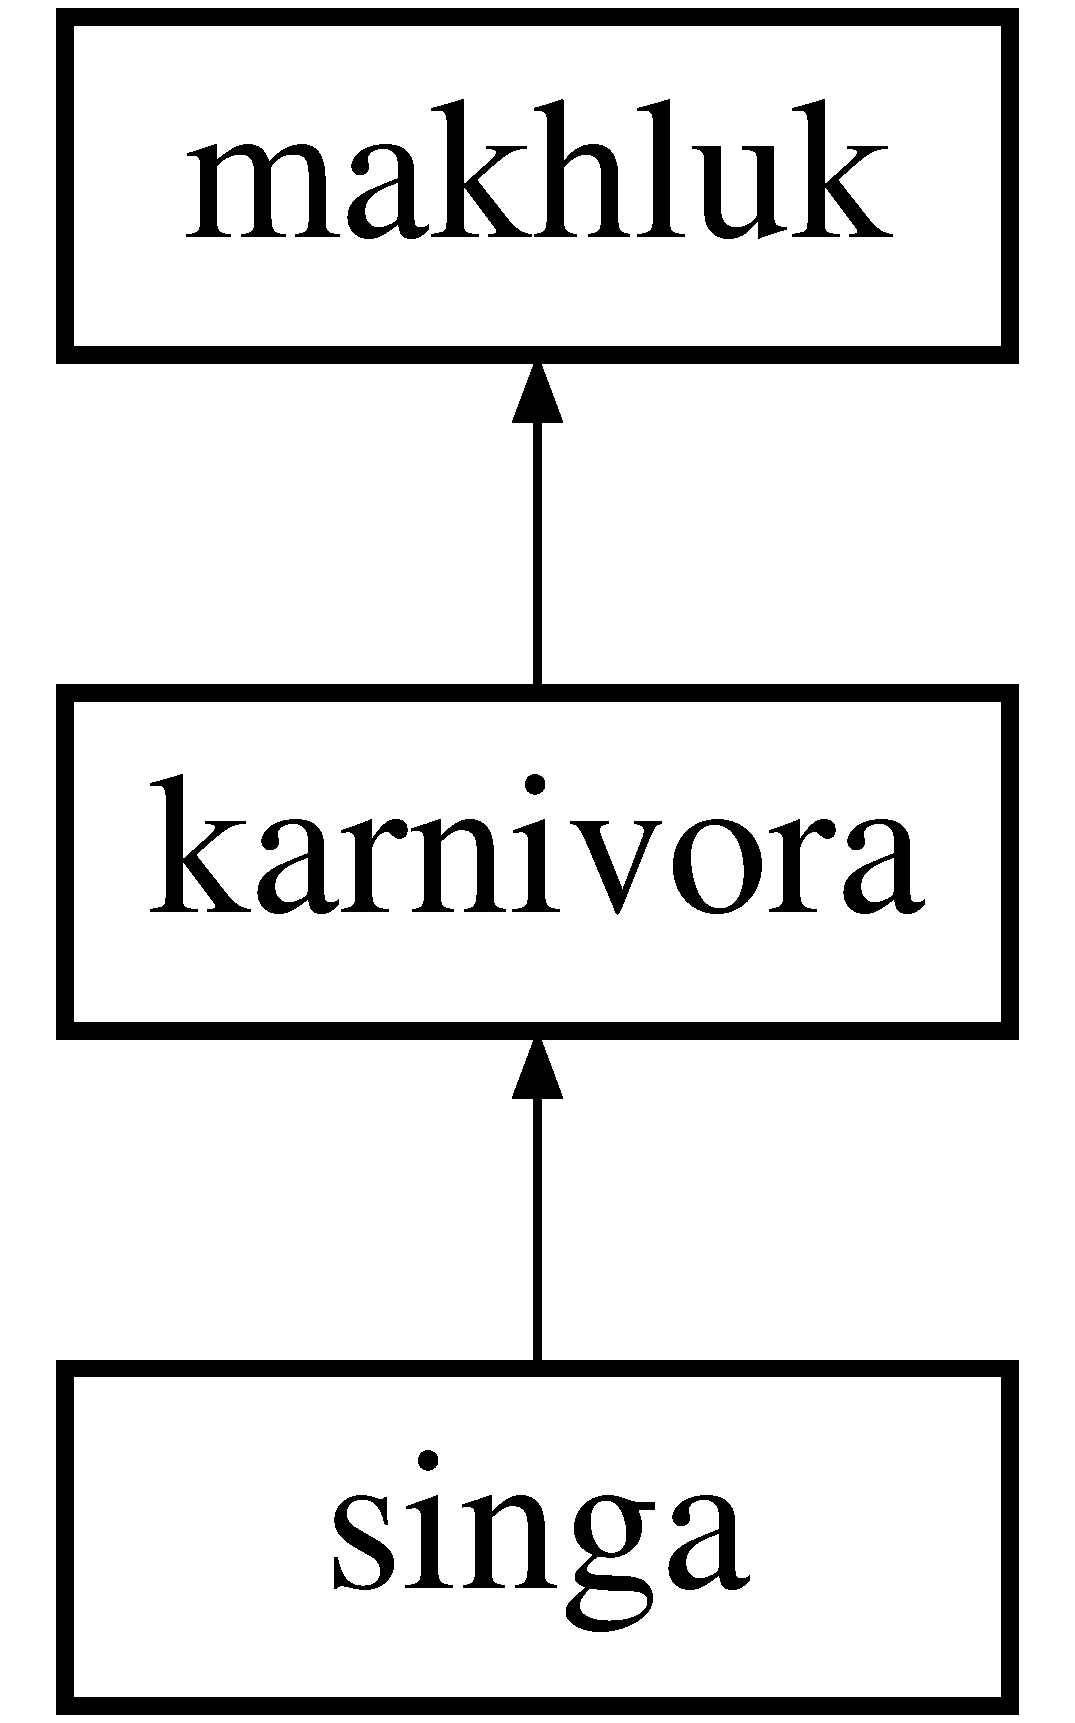
\includegraphics[height=3.000000cm]{classsinga}
\end{center}
\end{figure}
\subsection*{Public Member Functions}
\begin{DoxyCompactItemize}
\item 
{\bfseries singa} (\hyperlink{classsinga}{singa} \&)\hypertarget{classsinga_a4c15695e0ccf73ec7e45545cdb420d95}{}\label{classsinga_a4c15695e0ccf73ec7e45545cdb420d95}

\item 
\hyperlink{classsinga}{singa} \& {\bfseries operator=} (\hyperlink{classsinga}{singa} \&)\hypertarget{classsinga_ad7b992e78a1eefb92f515f646a8deb9b}{}\label{classsinga_ad7b992e78a1eefb92f515f646a8deb9b}

\item 
virtual void \hyperlink{classsinga_a5088d05298bfa251e2a6b8639ccff87a}{makan} ()\hypertarget{classsinga_a5088d05298bfa251e2a6b8639ccff87a}{}\label{classsinga_a5088d05298bfa251e2a6b8639ccff87a}

\begin{DoxyCompactList}\small\item\em memakan objek lain -\/ kelas turunannya harus mengimplementasikan ini \end{DoxyCompactList}\end{DoxyCompactItemize}
\subsection*{Protected Attributes}
\begin{DoxyCompactItemize}
\item 
const int {\bfseries maxlapar} = 30\hypertarget{classsinga_ad887e004abb6137c979cd381bb0b1913}{}\label{classsinga_ad887e004abb6137c979cd381bb0b1913}

\end{DoxyCompactItemize}


The documentation for this class was generated from the following files\+:\begin{DoxyCompactItemize}
\item 
singa.\+h\item 
singa.\+cpp\end{DoxyCompactItemize}

\hypertarget{classzebra}{}\section{zebra Class Reference}
\label{classzebra}\index{zebra@{zebra}}
Inheritance diagram for zebra\+:\begin{figure}[H]
\begin{center}
\leavevmode
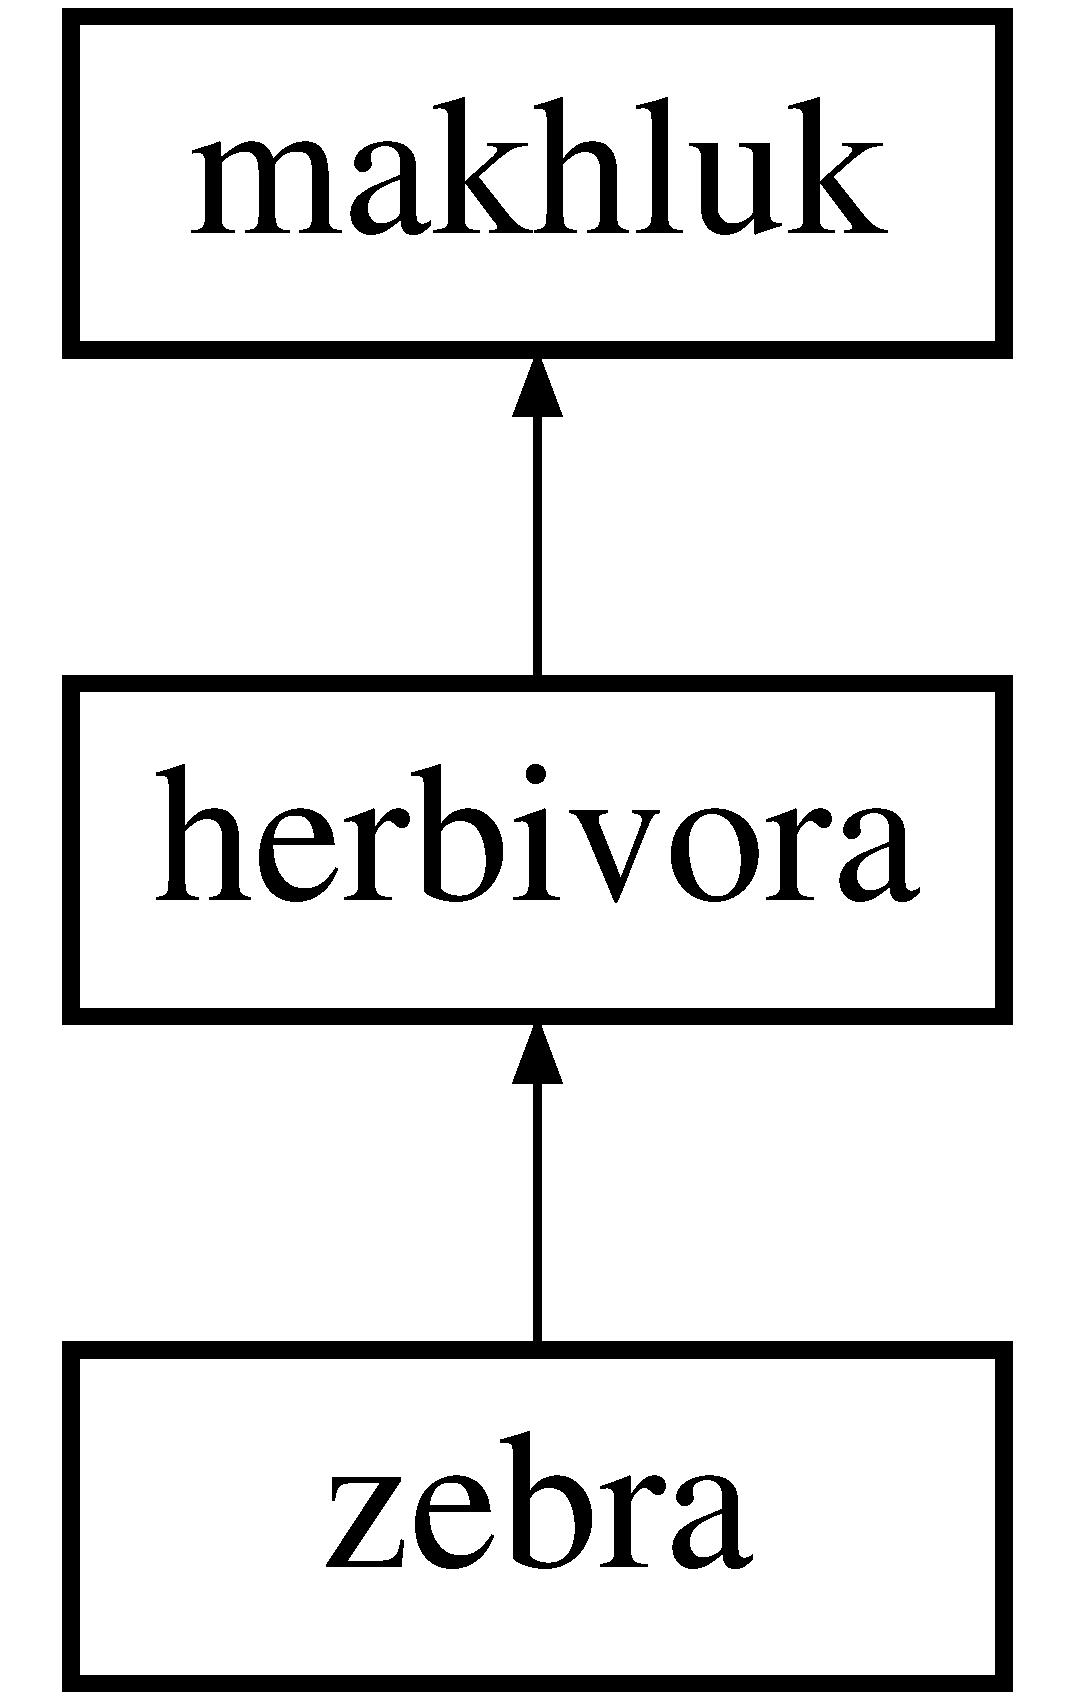
\includegraphics[height=3.000000cm]{classzebra}
\end{center}
\end{figure}
\subsection*{Public Member Functions}
\begin{DoxyCompactItemize}
\item 
virtual void \hyperlink{classzebra_ab9083f6b8691e987cde895d07d67da63}{makan} ()\hypertarget{classzebra_ab9083f6b8691e987cde895d07d67da63}{}\label{classzebra_ab9083f6b8691e987cde895d07d67da63}

\begin{DoxyCompactList}\small\item\em memakan objek lain -\/ kelas turunannya harus mengimplementasikan ini \end{DoxyCompactList}\end{DoxyCompactItemize}
\subsection*{Protected Attributes}
\begin{DoxyCompactItemize}
\item 
const int {\bfseries maxlapar} = 30\hypertarget{classzebra_aeca9f79d6791d93fc6e2faef9e52433d}{}\label{classzebra_aeca9f79d6791d93fc6e2faef9e52433d}

\end{DoxyCompactItemize}


The documentation for this class was generated from the following files\+:\begin{DoxyCompactItemize}
\item 
zebra.\+h\item 
zebra.\+cpp\end{DoxyCompactItemize}

%--- End generated contents ---

% Index
\backmatter
\newpage
\phantomsection
\clearemptydoublepage
\addcontentsline{toc}{chapter}{Index}
\printindex

\end{document}
